\documentclass[a4,oneside]{article}
\usepackage[colorlinks=true,linkcolor=blue,citecolor=blue]{hyperref}
\usepackage{natbib}
\usepackage{times}
\usepackage{listings}
\usepackage[table]{xcolor}
%\PassOptionsToPackage{table}{xcolor}
\usepackage{color}
%\usepackage{colortbl}
\usepackage{marginnote}
\usepackage{rotating}
\usepackage{lipsum}
\usepackage{longtable}
\usepackage{array}
\usepackage{amsmath}
\usepackage{mdframed,lipsum}
\usepackage{graphics}
% Set math in Times Roman
\DeclareSymbolFont{letters}{OML}{ptmcm}{m}{it}
\DeclareSymbolFont{operators}{OT1}{ptmcm}{m}{n}
%\DeclareSymbolFont{bold}     {OML}{ptmcm}{b}{it}
\DeclareMathAlphabet{\mathbf}{OT1}{ptm}{b}{n}
% Page set up
\setlength{\oddsidemargin}{0cm} %{0.5cm}
\setlength{\evensidemargin}{0cm} %{0.5cm}
\setlength{\topmargin}{-2cm}
\setlength{\textheight}{24cm}
\setlength{\textwidth}{16cm}
\setlength{\marginparsep}{0.5cm}
\setlength{\marginparwidth}{0cm}
\setlength{\parindent}{1em}
\setlength{\parskip}{0cm}
\renewcommand{\baselinestretch}{1.1}
\sloppy

% Configure appearance of code listings
\definecolor{light-gray}{gray}{0.92}
\def\codesize{\small}
\lstset{language=sh,
  backgroundcolor=\color{light-gray},
  numbersep=5pt,
  xleftmargin=0cm,
  xrightmargin=0cm,
  basicstyle=\footnotesize\ttfamily,
  emphstyle=\bfseries\color{red}}
\lstset{showstringspaces=false}

% Page headers
\usepackage{fancyhdr}
\pagestyle{fancy}
\renewcommand{\headrulewidth}{0.5pt}
\renewcommand{\sectionmark}[1]{\markright{\thesection.\ #1}}
\renewcommand{\subsectionmark}[1]{}
\fancyhead[RO,RE]{\thepage}
\fancyfoot[C]{}

% Symbols and macros
\newcommand{\ecckd}{ecCKD}
\newcommand{\Ecckd}{ECCKD}
\def\codesize{\small}
\def\code#1{{\codesize\texttt{#1}}}

% Title material
\title{The ECMWF Correlated K-Distribution Tool (ecCKD): \\ User Guide}

\author{Robin J. Hogan\\ \emph{European Centre for Medium Range
    Weather Forecasts, Reading, UK}}

\date{Document version 1.1 (January 2022) applicable to 
  \ecckd\ version 1.1\thanks{This document is copyright
    \copyright\ 2021-- ECMWF. If you have any queries about
    \ecckd\ that are not answered by this document
%
%or by the information on the \spsurf\ web site
%(\url{http://www.met.reading.ac.uk/clouds/spartacus})
%
    then please email me at
    \href{mailto:r.j.hogan@ecmwf.int}{\texttt{r.j.hogan@ecmwf.int}}.}}
\begin{document}
\maketitle

\section{Introduction}
\Ecckd\ is a software tool for generating gas-optics models based on
the correlated $k$-distribution (CKD) technique, for use atmospheric
radiation schemes. The tool offers the user complete flexibility in
which gases to represent, the concentration and pressure ranges to
cover, and how much accuracy is required (at the expense of
efficiency). It has, however, only been tested on terrestrial
atmospheres.  The resulting gas optics models are encoded in a
\emph{ckd-definition} file in self-describing netCDF format,
which can be read by the ecRad radiation scheme
\citep{Hogan&2018}. The idea of flexibly defining a gas-optics model
entirely by a single file originates with \cite{Edwards&1996}

Running the tool consists of performing a sequence of tasks in the
form of C++ executables, each of which reads a netCDF file (or files)
produced by the previous task, and generates a netCDF file to pass on
to the next. The complete chain of tasks may be controlled by shell
scripts, and the ones provided as part of this package are designed
for the case of generating multiple gas-optics models, enabling the
user more easily to sample the relationship between efficiency and
accuracy.

The spectroscopy used by \ecckd\ consists of the large dataset
produced as part of the Correlated K-Distribution Model
Intercomparison Project (CKDMIP), described by \cite{Hogan&2020},
which contains layer optical depth of nine gases (H$_2$O, O$_3$,
N$_2$, O$_2$, CO$_2$, CH$_4$, N$_2$O, CFC-11 and CFC-12) for a number
of atmospheric profiles computed using LBLRTM version
12.8. Line-by-line radiative transfer calculations are performed on
these spectra as part of the generation of new gas-optics models, but
no new spectra are generated.

Section \ref{sec:installation} outlines how to install \ecckd\ and its
prerequisites on your system. Section \ref{sec:scripts} describes how
to run \ecckd\ using the pre-written scripts and how to alter the
configuration. Section \ref{sec:license} summarizes the copyright
and license situation.

\section{Installation}
\label{sec:installation}
The code should work with most flavours of Linux and Unix. Please note
that you need the best part of 1 TB of disk space, mostly for the
CKDMIP dataset on which \ecckd\ depends.
\subsection{Prerequisites}
\begin{itemize}
\item The scripts explicitly use the Bourne Again shell (\code{bash})
  which is available on all Linux distributions but may be missing on
  some versions of Unix. It may be safe to simply replace this by the
  Bourne or Korn shell (\code{sh} or \code{ksh}) at the top of each
  script, but this has not been tested.
\item You will need a Fortran compiler that supports the 2003
  standard, and a C++ compiler that supports the 2011 standard
  (C++11).  I recommend installing the latest version of the GNU
  Compiler Collection (GCC) available for your platform and using
  \code{gfortran} and \code{g++}.
\item You will need to install the netCDF library, version 4 or later,
  including the Fortran interface. This needs to be the development
  version, i.e.\ including header files; packages to install on a
  Linux system may be called \code{libnetcdff-dev} or
  \code{libnetcdff-devel}. Version 4 is required to support the latest
  format, which is actually HDF-5 and supports very large arrays and
  data compression. Both CKDMIP and \ecckd\ use this format for large
  files and give them the \code{h5} suffix, while using the classic
  netCDF-3 format for smaller files (suffix \code{nc}). Both can be
  read by the netCDF-4 library.
\item You need the NCO tools to be installed on your system; these are
  a collection of command-line utilities for manipulating netCDF
  files.
\item Install the Adept library, version 2.1 or later
  \citep{Hogan2014}, from
  \url{http://www.met.reading.ac.uk/clouds/adept2} or
  \url{https://github.com/rjhogan/Adept-2}. This provides array,
  automatic-differentiation and minimization capabilities. You will
  need BLAS and LAPACK capabilities to be enabled; the Adept build
  system should find default versions of these libraries on your
  system if they are available, and while they won't be fast, they are
  adequate for \ecckd\ since matrix multiplication and linear algebra
  do not comprise a particularly large part of the computational cost
  of \ecckd.  Nonetheless, if you need to install a BLAS/LAPACK
  library then I recommend OpenBLAS. If you have the choice then I
  suggest you turn off OpenMP parallelization of BLAS matrix
  operations, since \ecckd\ uses OpenMP parallelism at a higher level.
\item Compile the CKDMIP software package available from the CKDMIP
  home page at \url{https://confluence.ecmwf.int/display/CKDMIP}.
\end{itemize}

\subsection{Compiling \ecckd}
The \ecckd\ software uses the autotools build system.  If you obtained
the software from GitHub, you will need to have autotools installed on
your system, with which you can generate the \code{configure} script
via
%
\begin{lstlisting}
 autoreconf -i
\end{lstlisting}
%
Then create Makefiles for your system with
%
\begin{lstlisting}
 ./configure
\end{lstlisting}
%
If you installed Adept in a nonstandard location, or you wish to use
particular C++ compiler options, you can do so as follows:
%
\begin{lstlisting}
 ./configure --with-adept=/home/robin/apps/adept-2.1 \
      CXXFLAGS="-Wall -g -O2 -march=native -std=c++11 -DADEPT_FAST_EXPONENTIAL"
\end{lstlisting}
%
Please note that if your C++ compiler does not use the C++11 standard
by default, you will need to specify it on the command line
(e.g.\ using the \code{-std=c++11} option for GCC above).

Finally, you can build the software with
\begin{lstlisting}
 make
\end{lstlisting}
%
This should generate numerous executables in the \code{src/ecckd}
directory. While these can probably be installed somewhere with
\code{make install}, the \ecckd\ pacakge has so far only been tested
by running from within its build directory.

To compule with debugging enabled, do a \code{make clean} then rerun
the \code{configure} script with optimizations turned off, bounds
checking of array operations and initialization of arrays with
signaling NaNs, as follows
%
\begin{lstlisting}
 ./configure CXXFLAGS="-Wall -g -O0 -std=c++11 -DADEPT_BOUNDS_CHECKING -DADEPT_INIT_REAL_SNAN"
\end{lstlisting}
%


\subsection{Installing CKDMIP datasets}
\label{sec:datasets}
\Ecckd\ requires the CKDMIP \emph{MMM}, \emph{Idealized} and
\emph{Evaluation-1} datasets, which are available from
\code{ftp://dissemination.ecmwf.int}, username \code{ckdmip}, password
available on request from Robin Hogan
(\code{r.j.hogan@ecmwf.int}). The total volume of the dataset is of
order 700 GB. Since much of the wall-clock time running \ecckd\ is
actually spent reading data from disk, you may find better performance
installing on a locally mounted drive rather than a network drive. If
the data are installed on your system in the
\code{\$CKDMIP\_DATA\_DIR} directory, then the following
subdirectories should be used:
\begin{lstlisting}
 $CKDMIP_DATA_DIR/mmm/conc
 $CKDMIP_DATA_DIR/mmm/lw_spectra
 $CKDMIP_DATA_DIR/mmm/sw_spectra
 $CKDMIP_DATA_DIR/idealized/conc
 $CKDMIP_DATA_DIR/idealized/lw_spectra
 $CKDMIP_DATA_DIR/idealized/sw_spectra
 $CKDMIP_DATA_DIR/evaluation1/conc
 $CKDMIP_DATA_DIR/evaluation1/lw_spectra
 $CKDMIP_DATA_DIR/evaluation1/sw_spectra
 $CKDMIP_DATA_DIR/evaluation1/lw_fluxes
 $CKDMIP_DATA_DIR/evaluation1/sw_fluxes
\end{lstlisting}

In addition to installing datasets from the FTP site above, you will
need to edit and run several scripts from in the \code{work/sw}
directory of the CKDMIP software package; these are
\code{make\_rayleigh\_evaluation.sh}, \code{make\_rayleigh\_mmm.sh},
\code{make\_ssi\_evaluation.sh} and \code{make\_ssi\_mmm.sh}. They
create files containing the Rayleigh layer optical depth and the solar
spectral irradiance for the \emph{Evaluation-1} and \emph{MMM}
datasets, and place them in the \code{sw\_spectra} directories
above. You will need to edit these scripts to ensure that the files
are put in the right place.

The \code{evaluation1/lw\_fluxes} and \code{evaluation1/sw\_fluxes}
subdirectories ought to contain files of the precomputed fluxes for
each of the CKDMIP scenarios described by \cite{Hogan&2020}, in each
of the narrow CKDMIP bands. Note that two versions may be available in
the longwave: those computed using one zenith angle per hemisphere are
named \code{*\_fluxes\_*}, while those computed using four zenith
angles per hemisphere are named \code{*\_fluxes-4angle\_*}. Only the
former can be used for training. To regenerate these files if needed,
you will need to edit and run the
\code{work/lw/run\_lw\_lbl\_evaluation.sh} and/or the
\code{work/sw/run\_sw\_lbl\_evaluation.sh} scripts in the CKDMIP
software package. Please note that this typically takes 1--2 days.

\subsection{Locating executables and datasets}
Assuming you will be using the scripts in the \code{test} directory
(or your own variants of them), you will need to edit the script
variables in the \code{test/config.h} file to point to executables and
directories containing CKDMIP datasets needed in the operation of
\ecckd. Specifically the following variables need to be set:
\begin{lstlisting}
 CKDMIP_DATA_DIR  # Top-level directory for the CKDMIP dataset
 CKDMIP_DIR       # CKDMIP software directory (executables in the bin subdirectory)
 BINDIR           # Location of the ecCKD executables
 WORK_DIR         # Location of a working directory for use by ecCKD
\end{lstlisting}

\section{Running \ecckd\ using scripts}
\label{sec:scripts}
\subsection{Performing additional line-by-line radiation calculations}
\label{sec:additional}
The files containing fluxes that were described in section
\ref{sec:datasets} consider all important gases and are used for part
of the optimization of the gas-optics models. However, the most
accurate way to treat minor greenhouse gases (CH$_4$, N$_2$O and the
CFCs) for climate applications has been found to be to create a
`composite gas' containing not only O$_2$ and N$_2$, but also the
minor greenhouse gases at present-day concentrations constant with
height; the optical properties of this composite gas are then treated
as a function of pressure and temperature alone. Variations in the
concentrations of the minor greenhouse gases are then treated using
\ecckd's \emph{relative-linear} representation, in which their optical
depth is assumed to be proportional to $(x-x_p)$, where $x$ is the
mole fraction of the gas and $x_p$ is the present-day mole
fraction. The optical depths due to each gas, including the composite
gas, are then summed. This approach is most accurate for
concentrations of the minor greenhouse gases close to present-day
values. See also section \ref{sec:create_lut}.

In order to train such a scheme, we first train the coefficients of
the major gases (H$_2$O, O$_3$ and CO$_2$) and the composite gas. This
requires reference line-by-line calculations for the
\emph{Evaluation-1} dataset in which the minor greenhouse gases are
constant with height.  However, the CKDMIP scenarios all use minor
greenhouse gas profiles that vary with height \citep[see Fig.\ 2
  of][]{Hogan&2020}. Therefore, we need to generate the fluxes for
several additional scenarios, which is achieved by running the
\code{run\_sw\_lbl\_evaluation.sh} and
\code{run\_lw\_lbl\_evaluation.sh} scripts in the \code{test}
directory. These scripts take several hours to complete, but will
generate files in the \code{\$WORK\_DIR/sw\_lbl\_fluxes} and
\code{\$WORK\_DIR/lw\_lbl\_fluxes} directories. The scenarios
generated have the tag \code{rel-*}, where \code{*} represents the
concentration of CO$_2$ in ppmv.

\subsection{Using the master scripts}
\label{sec:master}
The easiest way to run \ecckd\ is to use the scripts in the
\code{test} directory. The master scripts are \code{do\_all\_lw.sh}
and \code{do\_all\_sw.sh}, which perform all the steps necessary to
generate spectral definition files suitable for use in a radiation
scheme such as ecRad. They basically define three global variables to
configure the calculation, and then run further scripts in
sequence. The variables are as follows:
\begin{description}
\item[\code{APPLICATION}] -- This variable is set to one of
  \code{climate}, \code{global-nwp} or \code{limited-area-nwp}, and
  maps to the applications given in Table 1 of \cite{Hogan&2020}. It
  determines the range of greenhouse gas concentrations to train on
  (the NWP configurations being limited to present-day
  concentrations), and the minimum pressure at which heating rates
  will need to be simulated (limited-area NWP being 400~hPa and the
  other two being 2~hPa). The \code{check\_configuration.h} include
  script then uses the \code{APPLICATION} variable to define the
  \code{APP\_LOCAL} and \code{MIN\_PRESSURE} variables.
\item[\code{BAND\_STRUCTURE}] -- This variable consists of a
  space-separated list of strings describing the band structures that
  will be simulated.  In the longwave these may be \code{fsck}
  \citep[the full-spectrum correlated-$k$ method, FSCK, described
    by][]{Hogan2010}, \code{wide} or \code{narrow} \citep[the band
    structures proposed by][]{Hogan&2020}. In the shortwave the
  \code{wide} and \code{narrow} structures are available, plus
  \code{rgb} which uses FSCK in a large near-infrared band, three
  visible bands for red green and blue, and one ultraviolet band.  New
  band structures can be defined, but it requires defining a unique
  name for the structure and then editing numerous of the scripts so
  that the correct behaviour is then invoked. Furthermore, fluxes in
  each of the new bands need to be recomputed for the
  \emph{Evaluation-1} dataset in each scenario by editing and running
  the scripts described in section \ref{sec:datasets} and
  \ref{sec:additional}. Note that rerunning the scripts may not be
  needed if your band structure involves only groupings of the bands
  of an existing band structure (e.g.\ the \code{wide} CKDMIP band
  structure involves simply grouping the \code{narrow} CKDMIP bands);
  you will, however, need to edit the scripts
  (e.g.\ \code{optimize\_lut\_sw.sh}) to specify the
  \code{band\_mapping} variable for your new band structure.
\item[\code{TOLERANCE}] -- This variable consists of a space-separated
  list of numbers representing the heating-rate tolerance (in
  K~day$^{-1}$) used per spectral interval (g point), although note
  that the final accuracy of the scheme may differ considerably from
  this when gas overlap and other factors are accounted for.
\end{description}
If the scripts run successfully (which could take many hours),
spectral definition files will be written in the directory
\code{\$WORK\_DIR/sw\_ckd-definition} or
\code{\$WORK\_DIR/lw\_ckd-definition} with filenames of the form
\begin{lstlisting}
 ecckd-${VERSION}_sw_ckd-definition_${APPLICATION}_${BAND_STRUCTURE}-tol${TOLERANCE}.nc
 ecckd-${VERSION}_lw_ckd-definition_${APPLICATION}_${BAND_STRUCTURE}-tol${TOLERANCE}.nc
\end{lstlisting}
After running the complete chain of tasks, you may wish to rerun part
of the chain, which is simply a case of commenting out parts of the
master script and rerunning it, since the intermediate files will
still be present.

Figure \ref{fig:flowchart} depicts tasks that are performed, which are
described in more detail in sections
\ref{sec:merge}--\ref{sec:rt}. The detailed configuration settings for
each task are set in the individual scripts that enact these tasks,
and section \ref{sec:executables} outlines the general way in which
the executables are configured.  Note that these scripts are not
invoked directly by the user, but called from the master scripts
\code{do\_all\_lw.sh} and \code{do\_all\_sw.sh}.

\begin{figure}[tb!]
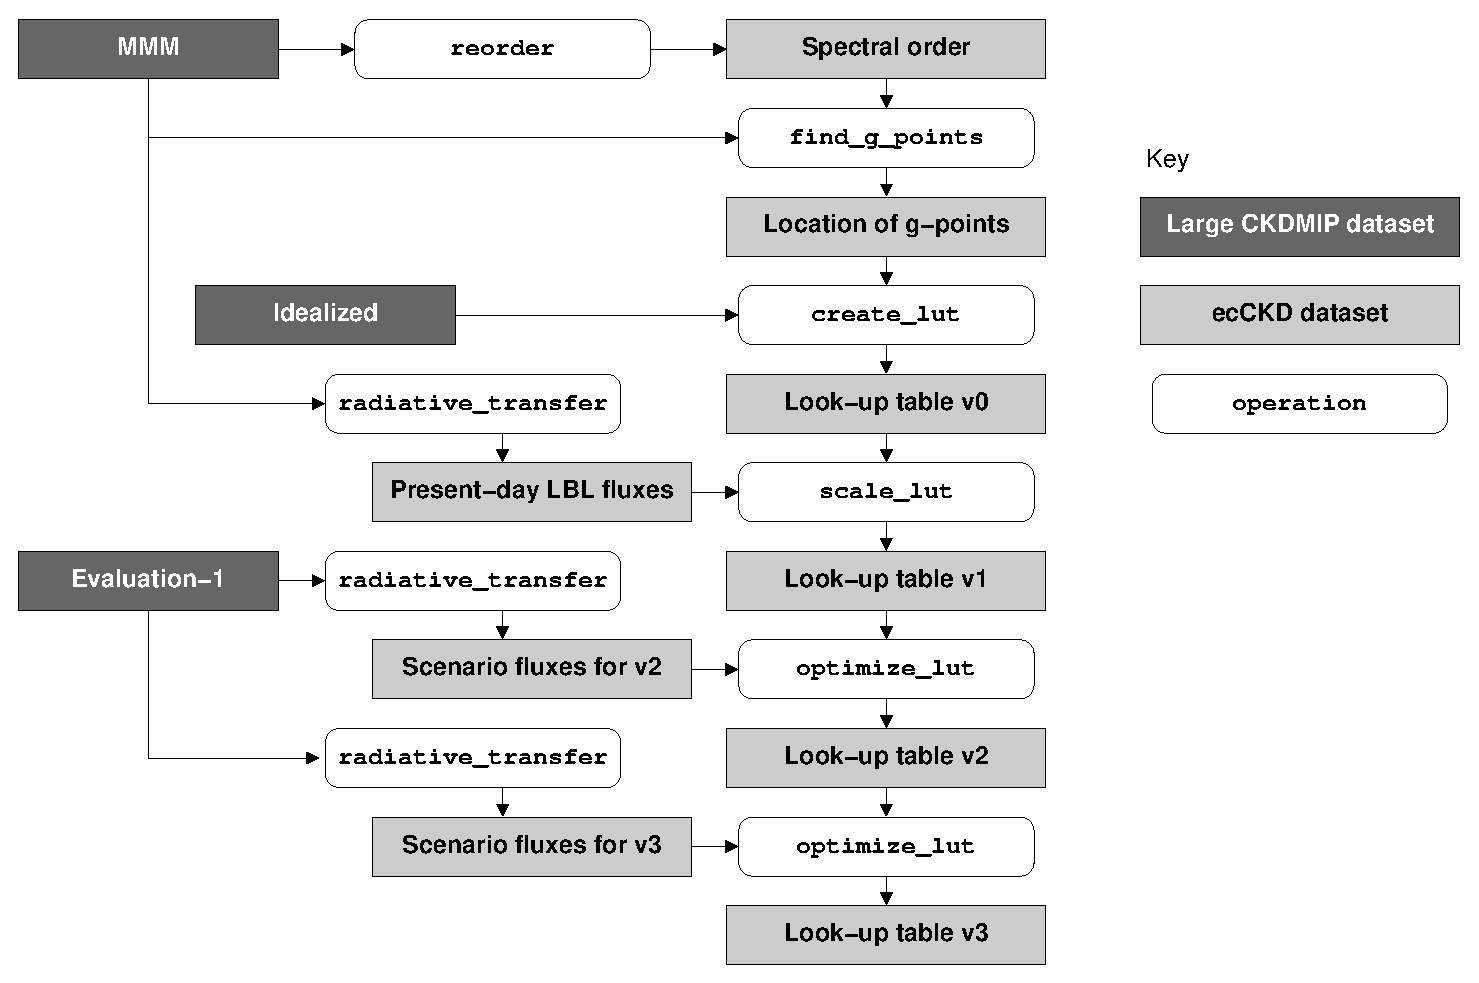
\includegraphics[width=\columnwidth]{flowchart.eps}
\caption{\label{fig:flowchart}Flowchart illustrating the tasks
  performed in generating an \ecckd\ spectral definition look-up
  table.}
\end{figure}

\subsection{Merging well-mixed gases}
\label{sec:merge}
The first task, not depicted in Fig.\ \ref{fig:flowchart}, is to merge
the absorption spectra of several combinations of gases for the
\emph{MMM} dataset. This is enacted by the
\code{merge\_well\_mixed\_lw.sh} and \code{merge\_well\_mixed\_sw.sh}
scripts, and the files are written to the
\code{\$WORK\_DIR/lw\_spectra} and
\code{\$WORK\_DIR/sw\_spectra}. This operation is done only once;
subsequent calls do nothing if the merged files are already
present. The intention is that when subsequent tasks need the combined
optical properties of common combinations of gases, they only need to
read one large file rather than several, but in practice only the
\code{reorder} task makes use of them, so this task may be removed in
a future version.

The merging is enacted by the \code{ckdmip\_lw} and \code{ckdmip\_sw}
executables from the CKDMIP software package.

\subsection{Reordering the spectra of individual gases}
The first task shown in Fig.\ \ref{fig:flowchart} is to reorder the
spectra of each gas in order of increasing absorption within each band
specified in \code{BAND\_STRUCTURE}, and is enacted by the
\code{reorder\_spectrum\_lw.sh} and \code{reorder\_spectrum\_sw.sh}
scripts (which in turn call the \code{reorder\_spectrum}
executable). This task is not repeated if the files are already
present. The median present-day profile from the \emph{MMM} dataset is
used. Ordering is in terms of the height of the peak cooling rate in
the longwave \citep[see][for details]{Hogan2010} and the height at
which the zenith optical depth reaches 0.25 when measured from
top-of-atmosphere in the shortwave. The latter figure can be set with
\code{threshold\_optical\_depth} in
\code{reorder\_spectrum\_sw.sh}. Thus \ecckd\ uses a unique mapping
from wavenumber to $g$-space, which is similar to the approach of
\cite{Doppler+2014} but differs from many CKD implementations that
reorder the spectra independently at each pressure level. We find the
unique mapping approach more attractive on physical grounds as it
avoids radiation implicitly changing its wavenumber as it passes
through the atmosphere, a property that is particularly important when
using very wide bands.

The resulting files are written to the \code{\$WORK\_DIR/lw\_order}
and \code{\$WORK\_DIR/sw\_order} subdirectories.  Note that the files
contain only the rank of each wavenumber, rather than full reordered
spectra themselves.

\subsection{Finding g points}
A correlated $k$-distribution model is efficient because it groups
together parts of the spectrum with similar absorption coefficient (`g
points'), even if they are not adjacent in wavenumber space, and
treats them with a single pseudo-monochromatic radiative transfer
calculation.  The \code{find\_g\_points\_lw.sh} and
\code{find\_g\_points\_sw.sh} scripts (which in turn call the
\code{find\_g\_points} executable) read in the spectral order of each
gas, and partition the spectra for each gas and band into g-points
such that a penalty function (quantifying the difference in heating
rate and fluxes between a quasi-monochromatic calculation for that
g-point and the line-by-line `truth') is below the specified
\code{TOLERANCE}. Thus, the lower the tolerance, the larger the number
of g-points that will be needed. Heating-rate and flux errors are
computed in the presence of other gases, but with their concentrations
set to the minimum for the specified \code{APPLICATION} \citep[for all
applications the minimum water vapour and ozone are taken from the
\emph{MMM} dataset, while for the climate application the greenhouse
gas concentrations are set to the minima of the scenarios listed in
Table 2 of][]{Hogan&2020}.  After working out the partitioning for
each individual gas, the gases are overlapped using the
hypercube-partition method of \cite{Hogan2010}.

\begin{table}[tb!]
\caption{\label{tab:find_g_points}General settings for the
  \code{find\_g\_points} executable, and the default values in the
  longwave and shortwave scripts.}
\begin{center}
\begin{tabular}{lcc>{\raggedright\arraybackslash}p{7cm}}
\hline
Setting & LW default & SW default & Description\\
\hline
averaging\_method & transmission & total-transmission & Method for averaging absorption coefficients to for candidate g points (other methods being `linear', `square-root' and `logarithmic' \\
tolerance\_tolerance & 0.01 & 0.01 & Fractional difference permitted between penalty functions for each g point \\
flux\_weight & 0.0 & 0.1 & Weight of fluxes relative to heating-rates in penalty function \\
max\_iterations & 60 & 60 & Maximum number of iterations when attempting to partition each band evenly into g points\\
iprofile & 0 & 0 & 0-based index of the profile to use from the \emph{MMM} dataset, 0 indicating the median profile\\
\hline
\end{tabular}
\end{center}
\end{table}

The configuration settings of the \code{find\_g\_points} executable
are quite complicated, since the treatment of each gas needs to be
specified separately. Some general settings are listed in Table
\ref{tab:find_g_points}, while an example of the more detailed
settings is given in section \ref{sec:executables}. The
\code{averaging\_method} deserves some comment; it determines how
absorption coefficients are averged in candidate g-points.  In the
longwave the \code{transmission} method conserves the layer
transmission and emission assuming the flux in each high-resolution
wavenumber is equal to the Planck function at the temperature of the
layer. In the shortwave, only the direct downward flux is computed,
and it is possible to construct an absorption profile for the g-point
such that a quasi-monochromatic direct-beam radiation calculation
reproduces the line-by-line direct-beam flux profile exactly. The
\code{total-transmission} averaging method does exactly this, but then
computes the penalty function by scaling the absorption of the gas
between the values specified by the gas-specific configuration
parameters \code{min\_scaling} and \code{max\_scaling}, intended to
represent the range of concentrations of that gas. Internally, these
scalings may be adjusted to span at least the range 0.5--2.5, since
that is required to represent the capture the large part of the
variation of the solar path length through the atmosphere over the
diurnal cycle.

A separate output file is written for each \code{BAND\_STRUCTURE} and
\code{TOLERANCE} in the \code{\$WORK\_DIR/lw\_gpoints} and
\code{\$WORK\_DIR/sw\_gpoints} directories.

\subsection{Initial creation of look-up table}
\label{sec:create_lut}
The \code{create\_lut\_lw.sh} and \code{create\_lut\_sw.sh} scripts
(which call the \code{create\_lut} executable) read in the CKDMIP
\emph{Idealized} dataset, and average the molar absorptions into each
g point. In the shortwave it also computes the Rayleigh scattering
contribution for each g point in the form of a single molar scattering
coefficient. This task is relatively slow because the entire
\emph{Idealized} dataset needs to be read in for each combination of
\code{BAND\_STRUCTURE} and \code{TOLERANCE}. The result is written to
the \code{\$WORK\_DIR/lw\_raw-ckd-definition} and
\code{\$WORK\_DIR/sw\_raw-ckd-definition} directories in the form of a
fully functioning spectral definition look-up table file that could in
fact be used directly in a radiation scheme like ecRad. In practice
this first estimate is not very accurate, and so the subsequent steps
perform refinements, as indicated by the increasing versions of the
look-up table file shown in Fig.\ \ref{fig:flowchart}.

The \code{conc\_dependence} configuration parameter for each gas
specifies one of several ways in which the concentration dependence is
to be represented:
\begin{description}
\item[\code{none}] -- This is used for composite gases that encompass
  the contribution from all gases that are assumed to have a constant
  mole fraction (although optionally varying with pressure). Thus the
  absorption (actually expressed as an absorption per mole of all
  gases present) in each g point is a function of temperature and
  pressure alone.
\item[\code{linear}] -- This is used for gases whose absorption scales
  linearly with concentration, and for terrestrial atmospheres this is
  a very good approximation for all gases except water vapour. Thus
  the molar absorption coefficient of the gas in each g point is a
  function of temperature and pressure alone.
\item[\code{relative-linear}] -- This is the same as linear except
  that when used in a radiation scheme, the molar absorption
  coefficient is not simply multiplied by the mole fraction of the
  gas, but by the mole fraction minus a reference value (specified by
  the \code{reference\_conc} parameter for that gas). See section
  \ref{sec:additional} for further information.
\item[\code{lut}] -- In this case the concentration dependence is
  represented by adding a concentration dimension to the look-up
  table. In terrestrial atmospheres this is needed only for water
  vapour.
\end{description}
Subsequent radiation schemes simply sum the optical depths of each
active gas in each g point.

\subsection{Shortwave scaling of look-up table}
The first refinement of the spectral description look-up table, only
performed in the shortwave, takes advantage of the fact that given a
profile of `true' line-by-line direct fluxes (for a solar zenith angle
of 60$^\circ$) for the spectral interval represented by each g point,
it is possible to define a profile of monochromatic layer optical
depths that reproduces this profile exactly. The
\code{scale\_lut\_sw.sh} script, which calls the \code{scale\_lut}
executable, does exactly this using line-by-line fluxes from the
CKDMIP median profile as the reference.  It then works out the scaling
that would be required, as a function of pressure, to correct the
optical depth profile (which represents all gases) coming out the v0
look-up table. It assumes that each gas has the same fractional error
in absorption, and scales the look-up tables for each gas by the same
pressure-dependent function. The new file is written to the same
directory but with the file specifier \code{scaled-ckd-definition}.

Before the scaling can be applied, the script creates a file
\begin{lstlisting}
 $WORK_DIR/sw_lbl_fluxes/ckdmip_mmm_sw_fluxes-raw_present_1.h5
\end{lstlisting}
(if not already present) containing the full spectral fluxes at all
altitudes for the first (median) profile of the \emph{MMM} dataset. It
uses the \code{ckdmip\_sw} executable from the CKDMIP package to do
this (and since this is coded in Fortran, a `1' is used in the file
name to indicate the first profile rather than `0').

\subsection{Optimization of coefficients}
The final part of the process is to optimize the look-up-table
coefficients by minimizing the difference between CKD and line-by-line
fluxes and heating rates for the 50 realistic profiles of the CKDMIP
\emph{Evaluation-1} dataset. For the climate application this is done
in several steps, first optimizing the major gases, then the minor
gases. Two steps are shown in Fig.\ \ref{fig:flowchart}. The
optimization steps required are specified in the space-separated
\code{OPTIMIZE\_MODE\_LIST} variable defined in the master scripts
discussed in section \ref{sec:master}. For each optimization step, the
\code{optimize\_lut\_lw.sh} and \code{optimize\_lut\_sw.sh} scripts
call the \code{optimize\_lut} executable, which generates a more
refined spectral-definition file (for each combination of
\code{BAND\_STRUCTURE} and \code{TOLERANCE}). The final files are
written to the \code{\$WORK\_DIR/sw\_ckd-definition} and
\code{\$WORK\_DIR/lw\_ckd-definition} directories.

\begin{table}[tb!]
\caption{\label{tab:optimize}General settings for the
  \code{optimize\_lut} executable, and the typical values (or range of
  values) used in the scripts.}
\begin{center}
\begin{tabular}{lc>{\raggedright\arraybackslash}p{9cm}}
\hline
Setting & Typical & Description\\
\hline
prior\_error & 2.0 & Error assigned to the prior values of the look-up table coefficients read in \\
broadband\_weight & 0.0--0.8 & Weight assigned to broadband fluxes and heating rates in the penalty function, as opposed to band fluxes; if this is non-zero then it allows errors in one band to be traded against errors in another which may or may not be desirable\\
flux\_weight & 0.01--0.3 & Weight of fluxes at TOA/surface to penalty function\\
flux\_profile\_weight & 0.05 & Weight of flux profile to penalty function \\
spectral\_boundary\_weight & 0.0--0.1 & Weight of fluxes in each g point at TOA/surface (rather than fluxes in each band), if available\\
temperature\_corr & 0.8 & Background error correlation between adjacent look-up table elements in the temperature dimension\\
pressure\_corr & 0.8  & Background error correlation between adjacent look-up table elements in the pressure dimension\\
conc\_corr & 0.8  & Background error correlation between adjacent look-up table elements in the concentration dimension\\
max\_iterations & 2000 & Maximum number of iterations to perform \\
convergence\_criterion & 0.0005--0.02 & Norm of the gradient of the penalty function at which convergence is deemed to have occurred \\
\hline
\end{tabular}
\end{center}
\end{table}

Internally, a quasi-Newton algorithm is used to minimize a penalty
function by adjusting all the look-up-table coefficients, provided by
the Adept package (since version 2.1). The main options governing the
behaviour of the optimization are provided in Table
\ref{tab:optimize}.

\subsection{Radiative transfer calculations using generated gas-optics models}
\label{sec:rt}
The final task carried out by the master scripts, but not shown in
Fig.\ \ref{fig:flowchart}, is to perform radiative transfer
calculations on the CKDMIP evaluation profiles for the various climate
scenarios, but using the gas-optics models generated by \ecckd. This
is enacted by the \code{run\_ckd\_lw.sh} and \code{run\_ckd\_sw.sh}
scripts. They first call the \code{run\_ckd} executable, which
generates files in the \code{\$WORK\_DIR/lw\_optical-depth} and
\code{\$WORK\_DIR/sw\_optical-depth} directories containing the layer
optical depths in each g point combining the contribution from all
gases.  These files are of the format required to participate in the
CKDMIP intercomparison. The scripts then call the \code{ckdmip\_lw}
and \code{ckdmip\_sw} executables from the CKDMIP package to compute
flux profiles, and write the results to the
\code{\$WORK\_DIR/lw\_fluxes} and \code{\$WORK\_DIR/sw\_fluxes}
directories. Both steps are very fast. These results may then be
compared statistically to the line-by-line fluxes for these profiles
to produce evaluation plots of the type shown in Fig.\ 5--8 of
\cite{Hogan&2020}.  Note that the \emph{Evaluation-1} profiles are not
independent as they are used in the training, but if the
\code{EVALUATION\_CODE} variable in the \code{test/config.h} include
script is set to \code{evaluation2} then the independent
\emph{Evaluation-2} dataset will be used instead, if available.

\subsection{Syntax for configuring \ecckd\ executables}
\label{sec:executables}
Each of the executables are configured in the same general way, making
use of the \code{readconfig} library provided in the \code{src/tools}
directory. The executables are all called in the same general way:
\begin{lstlisting}
 executable [key1=value1 [key2=value2 ...]] config.cfg
\end{lstlisting}
where \code{config.cfg} contains a list of key-value pairs. Additional
key-value pairs may be provided on the command-line as shown, and
override any matching keys in the configuration file. The values may
be scalars, arrays, strings or space-separated lists of strings. As an
example, the following configuration is written by the
\code{find\_g\_points\_lw.sh} script for the \code{global-nwp}
application, and passed to the \code{find\_g\_points} executable:
%
\begin{lstlisting}
# General configuration options
iprofile 0
averaging_method "transmission"
tolerance_tolerance 0.015
flux_weight 0.0
min_pressure 2.0
max_iterations 60

# List of gases to treat
gases composite h2o o3

# Detailed description of how individual gases are to be treated
\begin h2o
  # Water vapour in median present-day concentrations
  input ckdmip_mmm_lw_spectra_h2o_median.h5
  reordering_input lw_order_global-nwp_h2o.h5
  # Other gases in present-day concentrations, except ozone which uses
  # the minimum concentration
  background_input "ckdmip_mmm_lw_spectra_composite_present.h5
            ckdmip_mmm_lw_spectra_o3_minimum.h5"
\end h2o

\begin o3
  input ckdmip_mmm_lw_spectra_o3_median.h5
  reordering_input lw_order_global-nwp_o3.h5
  background_input "ckdmip_mmm_lw_spectra_composite_present.h5
            ckdmip_mmm_lw_spectra_h2o_minimum.h5"
\end o3

\begin composite
  input ckdmip_mmm_lw_spectra_composite_present.h5
  reordering_input lw_order_global-nwp_composite.h5
  background_input "ckdmip_mmm_lw_spectra_h2o_minimum.h5
            ckdmip_mmm_lw_spectra_o3_minimum.h5"
\end composite
\end{lstlisting}
Options could then be overridden on the command-line with
\begin{lstlisting}
 ./find_g_points gases="h2o o3" o3.input=alternative_o3_spectra.h5 config.cfg
\end{lstlisting}
Note that keys in sections in the configuration file are specified as
\code{SECTION.KEY} when given on the command-line.

\section{License and copyright}
\label{sec:license}
The \ecckd\ software in directory \code{src/ecckd} is copyright
\copyright\ 2019-- ECMWF. The software in the \code{src/tools} and
\code{src/include} is jointly owned by the University of Reading and
ECMWF; see the copyright statements in individual files. All the
software in these directories is licensed under the terms of the
Apache Licence Version 2.0 which can be obtained at
\url{http://www.apache.org/licenses/LICENSE-2.0}, and is also
available in the \code{LICENSE} file in the \ecckd\ package.  In
applying this licence, ECMWF does not waive the privileges and
immunities granted to it by virtue of its status as an
intergovernmental organisation nor does it submit to any jurisdiction.

\begin{thebibliography}{00}
%    
\bibitem[{Doppler et~al.(2014)}]{Doppler+2014}Doppler, L.,
  R. Preusker, R. Bennartz and J. Fischer, 2013: {k-bin} and {k-IR}:
  k-distribution methods without correlation approximation for
  non-fixed instrument response function and extension to the thermal
  infrared---Applications to satellite remote
  sensing. \textit{J. Quant.\ Spectrosc.\ Radiat.\ Transfer,}
  \textbf{133,} 382--395,
  \url{https://doi.org/10.1016/j.jqsrt.2013.09.001}.
%
\bibitem[{Edwards and Slingo(1996)}]{Edwards&1996}Edwards, J. M., and
  A. Slingo, 1996: Studies with a flexible new radiation code: 1.
  Choosing a configuration for a large-scale
  model. \textit{Q. J. R. Meteorol.\ Soc.,} \textbf{122,} 689--719,
  \url{https://doi.org/10.1002/qj.49712253107}.
%
\bibitem[{Hogan(2014)}]{Hogan2014}Hogan, R. J., 2014: Fast
  reverse-mode automatic differentiation using expression templates in
  C++.  \textit{ACM Trans.\ Mathematical Softw.,} \textbf{40,}
  26:1--16, \url{https://doi.org/10.1145/2560359}.
%
\bibitem[{Hogan(2010)}]{Hogan2010}Hogan, R. J., 2010: The
  full-spectrum correlated-$k$ method for longwave atmospheric
  radiation using an effective Planck
  function. \textit{J. Atmos.\ Sci.,} \textbf{67,} 2086--2100,
  \url{https://doi.org/10.1175/2010JAS3202.1}.
%
\bibitem[{Hogan and Bozzo(2018)}]{Hogan&2018}Hogan R. J., and
  A. Bozzo, 2018: A flexible and efficient radiation scheme for the
  ECMWF model. \emph{J. Adv.\ Modeling Earth Sys.,} \textbf{10,}
  1990--2008, \url{https://doi.org/10.1029/2018MS001364}.
%
\bibitem[{Hogan and Matricardi(2020)}]{Hogan&2020}Hogan, R. J., and
  M. Matricardi, 2020: Evaluating and improving the treatment of gases
  in radiation schemes: the Correlated K-Distribution Model
  Intercomparison Project (CKDMIP). \textit{Geosci.\ Model Dev.,}
  \textbf{13,} {6501--6521,}
  \url{https://doi.org/10.5194/gmd-13-6501-2020}.
%
\end{thebibliography}

\end{document}
